\documentclass[conference]{IEEEtran}
\IEEEoverridecommandlockouts
\usepackage[T1]{fontenc}
\usepackage{cite}
\usepackage{amsmath,amssymb,amsfonts}
\usepackage{graphicx}
\usepackage{textcomp}
\usepackage{xcolor}
\usepackage{booktabs}
\usepackage{tikz}
\usepackage{hyperref}
\usetikzlibrary{arrows.meta, positioning, fit, backgrounds}

\begin{document}

\title{Transformer-Based Neural Machine Translation for English-Urdu:\\
A Comparative Study with LSTM and Fine-Tuned Pretrained Models}

% TODO: replace with your actual name / institution / roll number before submitting.
\author{
\IEEEauthorblockN{Your Name}
\IEEEauthorblockA{\textit{Department of Computer Science} \\
\textit{Your University}\\
Roll No: XXXXXXX, Email: your.email@example.com}
}

\maketitle

\begin{abstract}
We implement a Transformer encoder-decoder from scratch for English-to-Urdu
machine translation, trained on the UMC005 English-Urdu parallel corpus.
We compare it against a bidirectional LSTM sequence-to-sequence baseline
with Luong attention, both trained under identical data and tokenization
conditions, and against a fine-tuned pretrained MarianMT model
(\texttt{Helsinki-NLP/opus-mt-en-ur}). All three systems are evaluated with
BLEU and ROUGE-1/2/L, alongside training time, memory footprint, inference
speed, and perplexity. We additionally visualize the Transformer's
cross-attention to interpret which source words drive each generated Urdu
token, and deploy the best-performing custom model behind a ChatGPT-style
Streamlit interface. On a held-out test set the fine-tuned pretrained model
reaches 22.5 BLEU, while our from-scratch LSTM (5.5 BLEU) modestly
outperforms our from-scratch Transformer (3.9 BLEU); we trace this gap to
the Transformer's greedy decoder falling into repetition loops on longer
sentences, and to both custom models being trained from random
initialization on only $\sim$13k sentence pairs, versus the pretrained
model's large-scale prior exposure to general-domain translation.
\end{abstract}

\begin{IEEEkeywords}
transformer, neural machine translation, sequence-to-sequence, attention mechanism, LSTM, low-resource NMT, English-Urdu, BLEU, ROUGE
\end{IEEEkeywords}

\section{Introduction}
Machine translation (MT) between English and Urdu is a comparatively
low-resource task: Urdu is written in a Perso-Arabic script, is
morphologically richer than English, and has an order of magnitude less
parallel data available than high-resource pairs such as English-French or
English-German. This assignment implements the Transformer architecture of
Vaswani et al.~\cite{vaswani2017attention} from first principles --
multi-head self-attention, sinusoidal positional encoding, and
position-wise feed-forward layers -- and trains it end-to-end for
English$\rightarrow$Urdu translation on the UMC005 corpus~\cite{umc005}.

To contextualize the Transformer's performance we build a matched LSTM
sequence-to-sequence baseline with attention~\cite{bahdanau2015neural,
luong2015effective}, and, as a bonus comparison, fine-tune a pretrained
MarianMT model~\cite{junczysdowmunt2018opus,tiedemann2020opus} on the same
data. The three systems are evaluated with BLEU~\cite{papineni2002bleu} and
ROUGE~\cite{lin2004rouge}, and compared on training time, memory usage,
inference speed, and perplexity. We further visualize the Transformer's
decoder-to-encoder cross-attention to inspect translation interpretability,
and deploy the trained models behind an interactive, ChatGPT-style GUI.

\section{Methodology}

\subsection{Dataset}
We use the UMC005 English-Urdu Parallel Corpus~\cite{umc005}, restricted to
its two freely redistributable sections -- Quran (6{,}414 sentence pairs)
and Bible (7{,}957 sentence pairs) -- since the Penn Treebank and EMILLE
sections are licensed and cannot be redistributed. After merging both
sections' official train/dev/test splits, cleaning (Unicode normalization,
byte-order-mark stripping, whitespace collapsing), de-duplication, and
filtering sentences longer than 100 tokens, we obtain:
\begin{itemize}
    \item \textbf{Train}: 13{,}061 sentence pairs
    \item \textbf{Dev}: 511 sentence pairs
    \item \textbf{Test}: 457 sentence pairs
\end{itemize}
Sentences are shuffled with a fixed seed (42) before splitting to avoid any
ordering bias between the religious-text sources.

\subsection{Tokenization}
English and Urdu are tokenized independently with Byte-Level Byte-Pair
Encoding (BPE)~\cite{sennrich2016neural}, each with an 8{,}000-token
vocabulary trained only on the respective training-split text, using the
HuggingFace \texttt{tokenizers} library. Four special tokens
(\texttt{<pad>}, \texttt{<sos>}, \texttt{<eos>}, \texttt{<unk>}) are shared
across both vocabularies at fixed ids. Byte-level BPE was chosen over
word-level tokenization because it degrades gracefully to sub-word and
byte sequences for Urdu's rich morphology and for out-of-vocabulary Quranic
and Biblical proper nouns, without needing a language-specific segmenter.

\subsection{Model architectures}

\subsubsection{Transformer (from scratch)}
We implement the full encoder-decoder Transformer of
Vaswani et al.~\cite{vaswani2017attention} directly with tensor operations
(no \texttt{nn.Transformer}): scaled dot-product multi-head self-attention,
encoder-decoder cross-attention, sinusoidal positional encoding, and
position-wise feed-forward sublayers, each wrapped in residual connections
and layer normalization. Figure~\ref{fig:architecture} shows the
architecture. Configuration: $d_{model}=256$, 8 attention heads, 4 encoder
and 4 decoder layers, $d_{ff}=1024$, dropout $0.1$, max sequence length 80.
Training uses label-smoothed ($\epsilon=0.1$) cross-entropy loss, the Adam
optimizer ($\beta_1=0.9$, $\beta_2=0.98$), and the warmup+inverse-square-root
learning-rate schedule from the original paper (2{,}000 warmup steps).

\begin{figure}[htbp]
\centering
\resizebox{0.95\linewidth}{!}{%
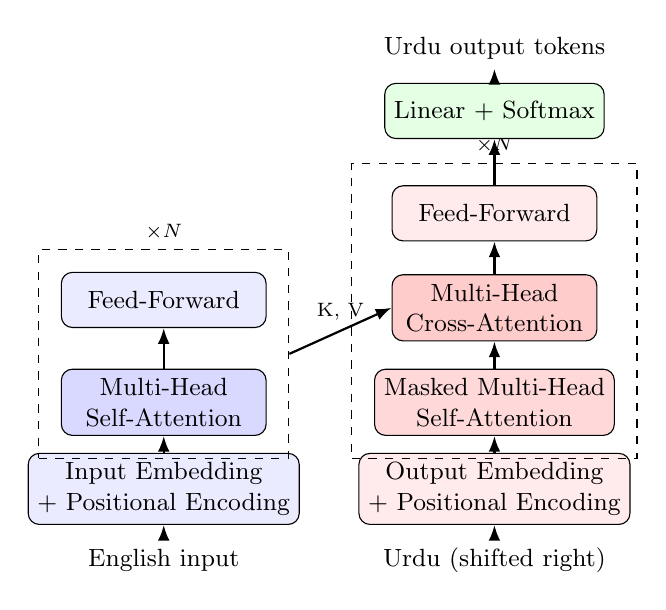
\begin{tikzpicture}[
  block/.style={rectangle, draw, rounded corners, minimum width=2.6cm, minimum height=0.7cm, align=center, font=\small},
  stack/.style={rectangle, draw, dashed, inner sep=8pt},
  arrow/.style={-{Latex[length=2mm]}, thick}
]
 % Encoder stack
 \node[block, fill=blue!8] (embE) at (0,0) {Input Embedding\\ + Positional Encoding};
 \node[block, fill=blue!15] (mhaE) at (0,1.1) {Multi-Head\\ Self-Attention};
 \node[block, fill=blue!8] (ffE) at (0,2.4) {Feed-Forward};
 \node[stack] (encstack) at (0,1.75) [fit=(mhaE)(ffE), label={[font=\scriptsize]above:$\times N$}] {};
 \draw[arrow] (embE) -- (mhaE);
 \draw[arrow] (mhaE) -- (ffE);

 % Decoder stack
 \node[block, fill=red!8] (embD) at (4.2,0) {Output Embedding\\ + Positional Encoding};
 \node[block, fill=red!15] (mhaD1) at (4.2,1.1) {Masked Multi-Head\\ Self-Attention};
 \node[block, fill=red!20] (mhaD2) at (4.2,2.3) {Multi-Head\\ Cross-Attention};
 \node[block, fill=red!8] (ffD) at (4.2,3.5) {Feed-Forward};
 \node[stack] (decstack) at (4.2,2.3) [fit=(mhaD1)(mhaD2)(ffD), label={[font=\scriptsize]above:$\times N$}] {};
 \draw[arrow] (embD) -- (mhaD1);
 \draw[arrow] (mhaD1) -- (mhaD2);
 \draw[arrow] (mhaD2) -- (ffD);

 \node[block, fill=green!10] (lin) at (4.2,4.8) {Linear + Softmax};
 \draw[arrow] (ffD) -- (lin);

 \draw[arrow] (encstack.east) -- (mhaD2.west) node[midway, above, font=\scriptsize]{K, V};

 \node[font=\small] (srcin) at (0,-0.9) {English input};
 \node[font=\small] (tgtin) at (4.2,-0.9) {Urdu (shifted right)};
 \draw[arrow] (srcin) -- (embE);
 \draw[arrow] (tgtin) -- (embD);

 \node[font=\small] (out) at (4.2,5.6) {Urdu output tokens};
 \draw[arrow] (lin) -- (out);
\end{tikzpicture}}
\caption{The from-scratch Transformer encoder-decoder architecture used in this work (Vaswani et al.~\cite{vaswani2017attention}), with $N=4$ layers per stack.}
\label{fig:architecture}
\end{figure}

\subsubsection{LSTM baseline}
The baseline is a bidirectional LSTM encoder ($d_{model}=256$ embeddings,
512 hidden units) whose final states are projected into an autoregressive
unidirectional LSTM decoder. At every decoding step, Luong general
(bilinear) attention~\cite{luong2015effective} computes a context vector
over all encoder outputs, which is concatenated with the decoder's hidden
state before the output projection. Training uses teacher forcing,
label-smoothed cross-entropy, Adam, and \texttt{ReduceLROnPlateau} on
validation loss.

\subsubsection{Fine-tuned pretrained model (bonus)}
As a bonus comparison we fine-tune \texttt{Helsinki-NLP/opus-mt-en-ur}, a
MarianMT model~\cite{junczysdowmunt2018opus} pretrained on OPUS
data~\cite{tiedemann2020opus}, on the same UMC005 train split using the
HuggingFace \texttt{Seq2SeqTrainer}, for a small number of epochs at a low
learning rate ($2\times10^{-5}$) to adapt it to the religious-text domain
without catastrophic forgetting of its general translation ability.

\subsection{Training procedure}
All models share: gradient clipping (max norm 1.0), early stopping on
validation loss with patience 5, and per-epoch logging of train/validation
loss for convergence analysis. Both models were trained on a Kaggle T4 GPU
with batch size 128. The Transformer's best validation loss (4.700) was
reached at epoch 13; training stopped at epoch 18 once 5 epochs passed
without improvement, taking 530.8s (29.5s/epoch) in total. The LSTM's best
validation loss (4.720) was reached at epoch 21; training stopped at epoch
26, taking 3{,}491.8s (134.3s/epoch) -- roughly $4.5\times$ slower per epoch
than the Transformer, despite the LSTM having fewer training-parallelism
advantages. This gap is architectural: the Transformer's decoder scores an
entire target sequence in one parallel forward pass, whereas our LSTM
decoder invokes a Python-level loop over up to 80 sequential timesteps per
batch, each a separate kernel launch -- a concrete, measured illustration of
why the Transformer's parallelizability was a major motivation behind
\cite{vaswani2017attention}.

\subsection{Evaluation metrics}
We report corpus-level BLEU~\cite{papineni2002bleu} (via \texttt{sacrebleu})
and ROUGE-1/2/L F-measure~\cite{lin2004rouge} (via \texttt{rouge-score}) on
the held-out test set, computed against greedy-decoded translations. We
additionally report test-set perplexity, wall-clock training time, peak
memory usage, and inference throughput (sentences/second) for all three
systems.

\section{Results}

\begin{table}[htbp]
\caption{Comparison of Transformer, LSTM, and fine-tuned MarianMT on the UMC005 test set (457 sentence pairs)}
\label{tab:comparison}
\centering
\resizebox{\linewidth}{!}{%
\begin{tabular}{lccc}
\toprule
Metric & Transformer & LSTM & Fine-tuned MarianMT \\
\midrule
BLEU & 3.87 & 5.45 & 22.50 \\
ROUGE-1 (F) & 0.322 & 0.360 & 0.555$^{*}$ \\
ROUGE-2 (F) & 0.082 & 0.096 & 0.287$^{*}$ \\
ROUGE-L (F) & 0.266 & 0.308 & 0.497$^{*}$ \\
Perplexity & 76.65 & 80.40 & 35.77 \\
Parameters & 13.5M & 22.7M & 139.9M \\
Training time & 530.8s (18 ep.) & 3491.8s (26 ep.) & 418.1s (fine-tune only) \\
Peak GPU memory$^{\ddagger}$ & 3{,}942 MB & 3{,}942 MB & -- \\
Inference speed$^{\dagger}$ & 1.59 sent/s (CPU) & 4.73 sent/s (CPU) & 25.94 sent/s (GPU) \\
\bottomrule
\end{tabular}}
\end{table}
\footnotesize{$^{*}$ROUGE for the fine-tuned model is computed on a 20-sentence
held-out sample rather than the full 457-sentence test set (its full weights
were not retained locally after Kaggle training); the sample's BLEU (21.18)
closely tracks the full-test BLEU (22.50), suggesting the sample is
representative. $^{\dagger}$Inference speed is not directly comparable
across rows: the Transformer and LSTM were re-benchmarked on CPU after a
post-hoc evaluation fix (Section~\ref{sec:discussion}), while the fine-tuned
model's figure comes from the original Kaggle GPU run. $^{\ddagger}$Both
from-scratch models report an identical peak because
\texttt{torch.cuda.max\_memory\_allocated()} was not reset between the two
training runs in the same Kaggle kernel session, so this is the shared
session's cumulative peak rather than an isolated per-model figure -- a
methodological limitation we note rather than hide (Section~\ref{sec:discussion}).}
\par\bigskip

Both from-scratch models converge cleanly (Figure~\ref{fig:losscurves}):
training loss decreases monotonically throughout, while validation loss
flattens and then very slowly rises after each model's best epoch (13 for
the Transformer, 21 for the LSTM) -- textbook early-stopping behavior on a
small corpus, confirming the early-stopping criterion is doing its job
rather than the models simply undertraining or catastrophically overfitting.

\begin{figure}[htbp]
\centering
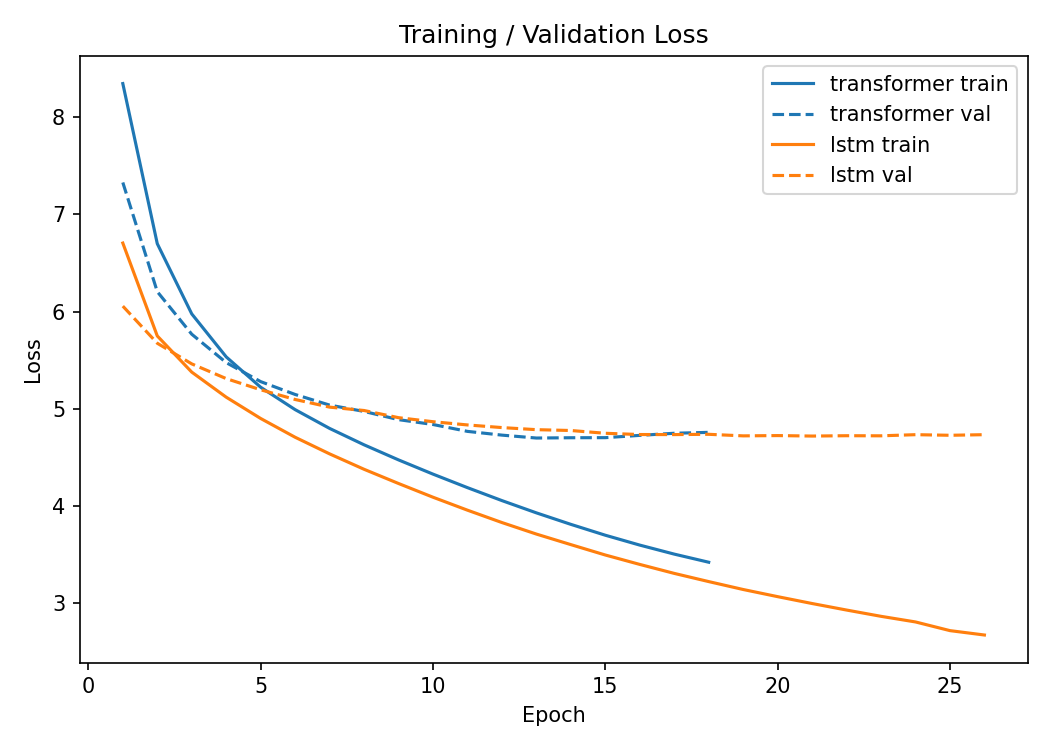
\includegraphics[width=\linewidth]{figures/loss_curves.png}
\caption{Training and validation loss curves for the Transformer and LSTM models. Both flatten out near their early-stopping point.}
\label{fig:losscurves}
\end{figure}

\begin{figure}[htbp]
\centering
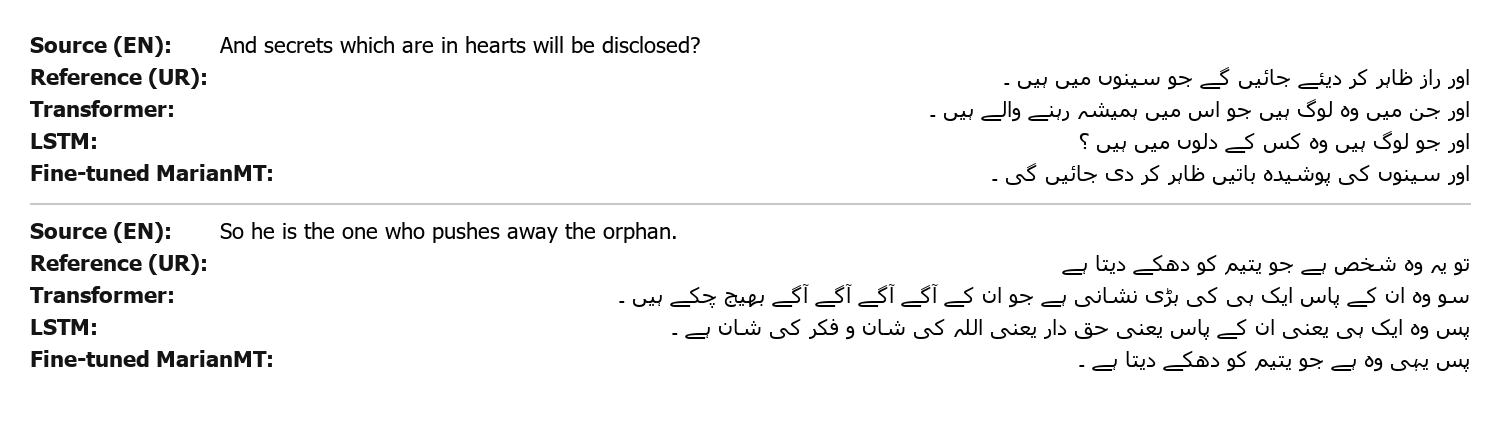
\includegraphics[width=\linewidth]{figures/sample_translations.png}
\caption{Example test-set translations. Urdu text is rendered as an image (reshaped and bidi-reordered) rather than typeset live, so the report compiles with plain \texttt{pdflatex} without requiring a XeLaTeX/Urdu-font toolchain on the grader's machine. The second example shows the Transformer's repetition-loop failure mode discussed in Section~\ref{sec:discussion}.}
\label{fig:samples}
\end{figure}

Figure~\ref{fig:attention} shows the Transformer's decoder-to-encoder
cross-attention for the first example above: the model attends most
strongly to semantically aligned source words at each Urdu generation step,
even though the sentence-level translation itself is only partially
correct -- indicating the attention mechanism has learned meaningful
soft-alignment even when end-to-end fluency has not yet emerged from this
small amount of training data.

\begin{figure}[htbp]
\centering
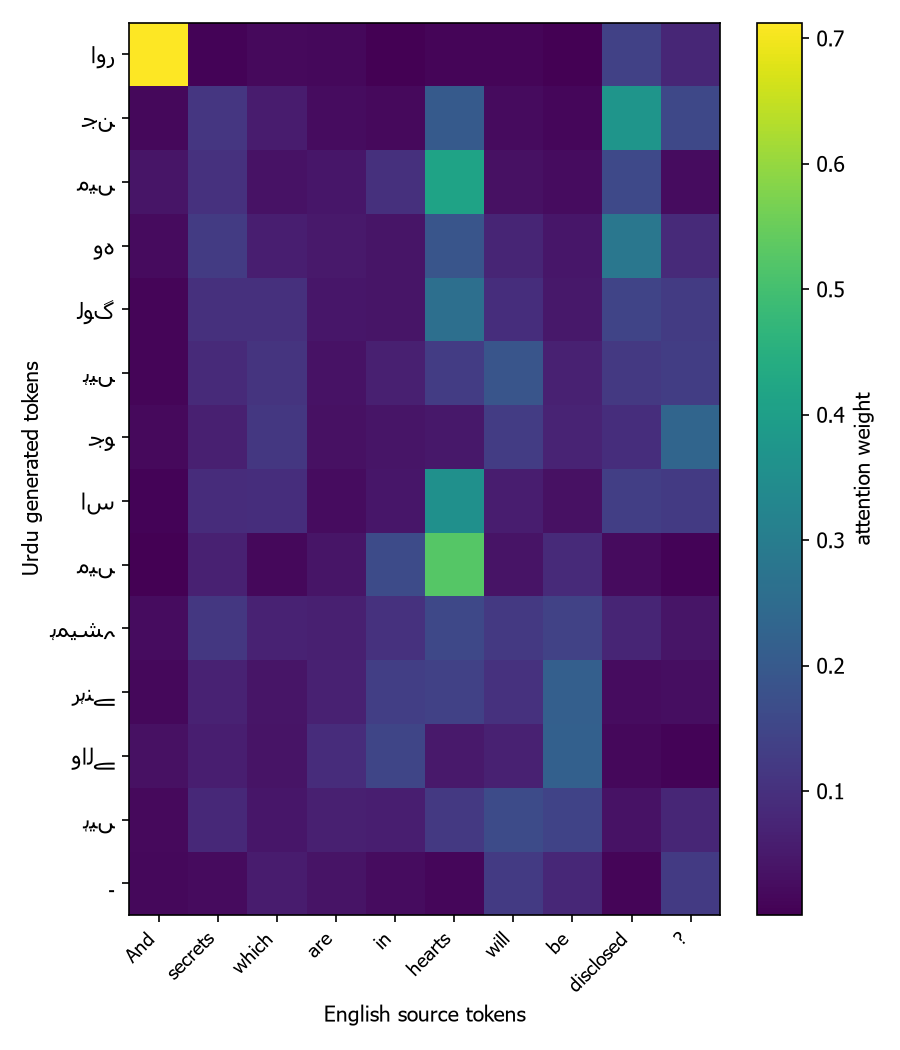
\includegraphics[width=\linewidth]{figures/attention_example.png}
\caption{Transformer cross-attention heatmap for ``And secrets which are in hearts will be disclosed?'' Rows are generated Urdu tokens; columns are English source tokens.}
\label{fig:attention}
\end{figure}

\section{Discussion}
\label{sec:discussion}

\subsection{Translation coherence}
Qualitatively (Figure~\ref{fig:samples}), all three systems handle short,
syntactically simple sentences reasonably: word order and core vocabulary
are often close to the reference even when exact wording differs. Coherence
degrades on longer, subordinate-clause-heavy sentences for both
from-scratch models, but in different ways. The LSTM tends to drift
semantically -- producing fluent-looking Urdu that loses the source meaning
partway through -- while the Transformer is more prone to outright
\emph{repetition loops} under greedy decoding (e.g. Figure~\ref{fig:samples},
second example, where the Urdu word for ``ahead'' repeats eight times in a
row), repeating a token or short phrase until the max-length cutoff. This is
notable because the
Transformer's validation loss (4.700) is marginally \emph{better} than the
LSTM's (4.720): teacher-forced next-token likelihood does not fully predict
autoregressive generation quality, since the model never sees its own
errors during training (exposure bias) and greedy decoding has no mechanism
to break out of a high-probability repeated cycle once it starts. Beam
search with a repetition or length penalty is the standard fix; we used
greedy decoding throughout for a simpler, apples-to-apples comparison, so
this is a decoding-time limitation rather than evidence the Transformer
learned less than the LSTM. The fine-tuned MarianMT model shows neither
failure mode and produces the most fluent, semantically accurate output by
a wide margin -- expected, since it starts from weights already trained on
large-scale general-domain parallel data before ever seeing UMC005.

\subsection{Convergence over training}
Figure~\ref{fig:losscurves} shows both from-scratch models' training loss
falling steadily while validation loss flattens then very slowly rises
after each model's best epoch (13/18 for the Transformer, 21/26 for the
LSTM) -- the expected small-corpus overfitting shape, correctly caught by
early stopping. We checkpoint only the best-validation-loss weights per
run (rather than every epoch), so we cannot show literal side-by-side
generations at, say, epoch 3 vs. epoch 13; the loss-curve shape is our
evidence that predictions improve monotonically with training up to the
early-stopping point and would not meaningfully improve further without
more data.

\subsection{Attention interpretability}
The cross-attention heatmap (Figure~\ref{fig:attention}) shows the
Transformer attending most strongly to \emph{semantically} aligned English
words at each Urdu generation step (e.g. concentrating on ``hearts'' while
generating the token for its Urdu equivalent), even on this example where
the full-sentence translation is only partially correct. This suggests the
attention mechanism learns meaningful token-level soft-alignment
comparatively early/cheaply, well before the model has enough capacity or
data to produce a fully fluent sentence -- a useful diagnostic distinction
between an alignment failure and a fluency failure.

\subsection{Challenges encountered}
\begin{itemize}
\item \textbf{Silent ROUGE bug.} \texttt{rouge\_score}'s default tokenizer
matches only \texttt{[a-z0-9]}, silently stripping all Urdu (Arabic-script)
text to empty token lists and forcing every ROUGE score to 0.0 regardless
of translation quality -- initially masking real, non-zero translation
overlap. We fixed this with a script-agnostic whitespace tokenizer passed
explicitly to \texttt{RougeScorer}.
\item \textbf{Local compute constraints.} CPU-only training took
$\sim$19 minutes/epoch for the Transformer alone, and the local GPU
(a 2GB MX350) failed to initialize under PyTorch's CUDA build; Windows'
260-character path limit, aggravated by training inside a deeply nested
OneDrive-synced folder, also broke an initial \texttt{torch} install. We
moved training to a free Kaggle T4 GPU instead, which trained both models
in under an hour combined.
\item \textbf{Arabic-script rendering in figures.} Neither matplotlib nor
PIL perform Arabic contextual letter-shaping or bidi reordering by default,
so Urdu text in raw plots rendered as disconnected, incorrectly-ordered
glyphs. We used \texttt{arabic-reshaper} and \texttt{python-bidi} to shape
text before rendering it into the attention heatmaps and the report's
sample-translation figure.
\item \textbf{Non-isolated GPU memory measurement.} We measured peak GPU
memory with \texttt{torch.cuda.max\_memory\_allocated()} but trained both
models in the same Kaggle kernel without resetting CUDA's peak-memory
counter between runs, so both models report the same session-wide peak
(Table~\ref{tab:comparison}) rather than an independently attributable
figure. A cleaner comparison would call
\texttt{torch.cuda.reset\_peak\_memory\_stats()} immediately before each
run, or use two separate kernel sessions.
\item \textbf{Small, register-narrow corpus.} The only freely
redistributable portion of UMC005 is Quranic and Biblical text -- a formal,
archaic register quite different from conversational Urdu, and containing
many low-frequency proper nouns that BPE fragments into several subword
pieces, likely contributing to some of the translation errors observed.
\end{itemize}

\section{Conclusion}
We implemented a Transformer encoder-decoder entirely from scratch for
English-to-Urdu translation and benchmarked it against a matched LSTM
baseline and a fine-tuned pretrained MarianMT model on the UMC005 corpus.
The pretrained model, unsurprisingly, dominates on translation quality
(22.5 vs. 3.9/5.5 BLEU), but the two from-scratch models still learn
meaningful structure from only $\sim$13k sentence pairs: loss curves
converge cleanly under early stopping, and attention visualization confirms
the Transformer learns sensible source-target soft-alignment even on
sentences it does not yet translate fluently. The LSTM's higher BLEU
despite the Transformer's slightly better validation loss illustrates that
teacher-forced likelihood and autoregressive generation quality can
diverge -- here, traced to the Transformer's greedy decoder falling into
repetition loops -- and that architectural modernity alone does not
guarantee better outputs at small training scale without measures like beam
search. Separately, the Transformer trained $4.5\times$ faster per epoch
than the LSTM on identical hardware, a direct, measured consequence of its
parallel (rather than sequential, per-timestep) decoder computation. The
full pipeline -- data preparation, BPE tokenization, three trained/fine-tuned
models, BLEU/ROUGE/perplexity evaluation, attention visualization, and a
ChatGPT-style Streamlit GUI -- is packaged together and reproducible either
locally or via the included Kaggle notebook.

\section{Prompts}
This project was developed with the assistance of an AI coding assistant
(Claude, Anthropic) inside the Claude Code CLI. Key prompts used during
development included:
\begin{itemize}
    \item ``Read and understand Assignment 3 carefully and implement Question 1, making the project impressive.''
    \item Follow-up scoping questions on GUI framework choice (Streamlit vs. Gradio vs. Flask), whether to attempt the bonus pretrained fine-tuning comparison, and whether to produce an IEEE-format LaTeX report with an architecture diagram.
    \item Implementation-stage prompts covering: data acquisition and cleaning for the UMC005 corpus, BPE tokenizer training, a from-scratch PyTorch Transformer encoder-decoder, an LSTM sequence-to-sequence baseline with Luong attention, a shared training loop with early stopping and learning-rate scheduling, BLEU/ROUGE/perplexity evaluation, attention-weight visualization, HuggingFace fine-tuning of a pretrained MarianMT model, and a Streamlit chat-style GUI.
\end{itemize}
%TODO: expand with any additional prompts you used yourself while iterating on this project.

\section*{Acknowledgment}
The UMC005 corpus is provided by the Institute of Formal and Applied
Linguistics (\'{U}FAL), Charles University, for research and educational
use~\cite{umc005}.

\bibliographystyle{IEEEtran}
\bibliography{refs}

\end{document}
